\documentclass{article}
\usepackage[slantfont,boldfont]{xeCJK}
\usepackage{ctex}
\usepackage{graphicx} % Required for inserting images
\usepackage[slantfont,boldfont]{xeCJK}
\usepackage{ctex}
\usepackage{graphicx} % Required for inserting images
\usepackage{geometry}
\usepackage{fancyhdr}
\usepackage{booktabs}
\usepackage{wasysym}
\usepackage{amsmath}
\usepackage[sort]{natbib}
\usepackage{indentfirst}
\usepackage[dvipdfm,  %pdflatex,pdftex    这里决定运行文件的方式不同
            pdfstartview=FitH,
            CJKbookmarks=true,
            bookmarksnumbered=true,
            bookmarksopen=true,
            colorlinks, %注释掉此项则交叉引用为彩色边框(将colorlinks和pdfborder同时注释掉)
            pdfborder=001,   %注释掉此项则交叉引用为彩色边框
            linkcolor=black,
            anchorcolor=black,
            citecolor=green
            ]{hyperref}
\geometry{left=2.54cm,right=2.54cm,top=3.18cm,bottom=3.18cm}
\newcommand{\chuhao}{\fontsize{42pt}{\baselineskip}\selectfont}
\newcommand{\xiaochuhao}{\fontsize{36pt}{\baselineskip}\selectfont}
\newcommand{\yihao}{\fontsize{28pt}{\baselineskip}\selectfont}
\newcommand{\erhao}{\fontsize{21pt}{\baselineskip}\selectfont}
\newcommand{\xiaoerhao}{\fontsize{18pt}{\baselineskip}\selectfont}
\newcommand{\sanhao}{\fontsize{15.75pt}{\baselineskip}\selectfont}
\newcommand{\sihao}{\fontsize{14pt}{\baselineskip}\selectfont}
\newcommand{\xiaosihao}{\fontsize{12pt}{\baselineskip}\selectfont}
\newcommand{\wuhao}{\fontsize{10.5pt}{\baselineskip}\selectfont}
\newcommand{\xiaowuhao}{\fontsize{9pt}{\baselineskip}\selectfont}
\newcommand{\liuhao}{\fontsize{7.875pt}{\baselineskip}\selectfont}
\newcommand{\qihao}{\fontsize{5.25pt}{\baselineskip}\selectfont}
\title{\vspace{-1.7cm}\textbf{华中科技大学未来技术学院\\《信号与系统》课程\\\vspace{3.5cm}
                        工程设计问题设计报告\\\vspace{3cm}题目:基于一维滤波器的图像处理\\\vspace{1.5cm}}}
\author{分组号:11\\组长:袁博文\\组员:时圣铭、孙鹏卓、王愉哲\\ 指导教师:庞元杰 }
\date{2023.5.25-2023.6.14}
\pagestyle{fancy}
\fancyhead[L]{\centering{华中科技大学未来技术学院《信号与系统》工程设计问题报告}}
\bibliographystyle{unsrt}
\begin{document}
\lhead{华中科技大学未来技术学院《信号与系统》工程设计问题报告}
\maketitle
\vspace{3cm}
\begin{center}
    报告日期:2023年5月25日
\end{center}
\newpage
\tableofcontents 

\newpage
\section{序言}
滤波器是一种选频装置,可以使信号中特定的频率成分通过,而极大地衰减其他频率成分。利用滤波器的选频作用,可以滤除干扰噪声或进行频谱分析。其中,一维数字滤波器是指是指处理的信号是单变量函数序列的滤波器,常用于信号处理、语音处理和图像处理等操作。一维滤波器通常由一个滤波器核或滤波器系数组成,其中的滤波器核是一个具有固定大小的一维数组,核中的每个元素表示滤波器在不同位置上的权重。通过将滤波器核应用于输入信号的不同位置,便可以计算输出信号在每个位置上的数值。它们用于对一维信号(例如时间序列或一维图像)进行滤波操作,通过改变信号中不同频率分量的振幅或相位来实现信号的增强或修改。

一维滤波器目前已经应用于语音处理,图像处理,生物信号处理等各个领域,同时也具有很高的实用性并可大大减少其计算效率。在语言处理方面,
Wei Yan 和 Jiashu Zhang提出了一种用于非线性语音预测的流水线神经IIR滤波器(PNIIR)\cite{YAN201864},很好地降低了计算的复杂度并维持了其性能。Srinivas, Nagapuri 和Pradhan提出了一种局部非均值的一维滤波器用于降噪,并应用在了语言处理方面\cite{article-speech}。Vinay Kumar 和 Sunil Bhooshan 设计了一种基于正交多项式的一维线性相位数字IIR滤波器\cite{article},得到了良好的截止特性,也获得了优秀的频率通带和过度的特性区域。在图像处理方面,Jongho Kim在处理图像的阻塞伪影问题时,提出的一维滤波器可自适应地缓解网格噪声,定向二维滤波器可减少楼梯噪声和对角线边缘附近的拐角异常值,同时保留原始细节。有着算法花费的运行时间更少的优点,因此可用于运动图像和静止图像的实时应用\cite{5174477}。韩思思,刘伟斌和邢薇薇三人在处理图像质量问题时,提出一种新的彩色图像照度增强技术来提高彩色图像的质量,对图像的增强效果显著\cite{8328477}。赵辉和余觉邦通过设计一种简单高效的可变分数延迟FIR滤波器,将该滤波器的计算复杂度降至仅与设计固定一维FIR的计算复杂度相当,虽然其只考虑一维FIR VFD滤波器,但将这种方法扩展到设计二维FIR VFD滤波器或其他类型的可变数字滤波器或会由更优的效果\cite{1593976}。Wei-Der Chang在研究FIR滤波器时提出了一种设计分数阶二维结构的新方法,利用DE算法求解二维FIR数字滤波器的脉冲响应使其相应的幅度响应可以满足期望的两个变量的分数阶微分器的幅度响应\cite{CHANG2009660}。在处理心电图信号(ECG)方面,Weitong Sun 和 Yuping Su的1D-ResCNN model 有效的提高了ECG图像处理的信噪比\cite{SUN2020108}。Ge Wang and Lin Yang在提出了一种深度因子分析的一维滤波器方法用于处理ECG信号,在降噪方面的效果十分显著\cite{WANG2020101824}。数字通信系统中,一维滤波器还常被用于信号调制、信道均衡和解调等环节,可以提高通信系统的性能,减少信号失真和噪声干扰。


而在我们的研究中,探索一维滤波器在处理图像方面的应用。图像可以被看作是一个二维信号,而一维滤波器可以应用于图像的每一行或每一列,从而实现对图像的滤波操作。于是,我们便可以采用一维滤波器来处理图像。

当将一维滤波器应用于图像的每一行时,可以对图像的水平方向进行滤波。这种滤波可以用于平滑图像、增强边缘、检测水平方向的特定模式等。类似地,将一维滤波器应用于图像的每一列时,可以对图像的垂直方向进行滤波,从而实现垂直方向的平滑、边缘增强或特定模式检测。一维滤波器在图像处理中具有计算效率高、方便、储存效率高等优点。

需要注意的是,一维滤波器也有一些限制。由于它们只能处理图像的行或列,一维滤波器无法捕捉到图像的全局特征。此外,在某些情况下,二维滤波器可能更适合处理具有复杂结构的图像。因此,在选择滤波器类型时,需要根据具体的应用场景和需求进行权衡。






\section{问题描述}
对于一维(1D)离散时间信号,可通过信号映射完成域变换,从而实现1D滤波器。而对于二维即更高维度的空间,完成响应的域变换则需要更多额外的计算和内存成本。为了避免这些额外成本,通常选择使用一维变换来执行二维滤波。


使用一维运算过滤二维信号的最常见方法是沿信号的每个维度执行单独的传递,即用两个用于不同方向的1D滤波器的级联来处理信号。一幅数字图像,是一个二维空间域离散信号,其每个像素的值对应该像素处信号的振幅。对于图像,可以沿每个图像行执行(水平)传递,并沿每个图像列执行(垂直)传递,从而完成二维离散时间信号的滤波。本设计所需图像见plus.mat。

1)使用matlab中函数butter和remez,通过滤波器的归一化截止频率Wc与滤波器的阶数n ,生成3个离散时间滤波器的系数: 
\begin{center}
Wc=0.4; n1=10; n2=4; n3=12; \\
$\left[b1,a1\right]= butter(n1,Wc)$; //对应巴特沃斯10阶滤波器\\
a2=1; b2=remez(n2, [0 Wc-0.04 Wc+0.04 1], [1 1 0 0]); //对应切比雪夫4阶滤波器\\
a3=1; b3=remez(n3, [0 Wc-0.04 Wc+0.04 1], [1 1 0 0]); //对应切比雪夫12阶滤波器\\
\end{center}


2)在matlab中绘制出上述三个滤波器频率响应的幅度谱与相位谱,对三个滤波器频率响应的幅值和相位进行考察。通过相位谱,观察哪个滤波器具有线性相位,即在同一周期内相位谱为一条直线。


3)以单位阶跃信号为输入,绘制出每个滤波器的阶跃响应。观察响应的最大值与稳态值的差值,判断哪个滤波器具有最大的超调。 


4)用image(64*x)画出图像x(在plus.mat中),使用三个滤波器分别对图像x进行行、列滤波。通过Matlab的filter函数进行列滤波;将图像转置后再通过filter滤波,之后再进行转置,得到行滤波的结果。比较哪个输出图像具有更多的振荡?


5)通过MSE与PNSR指标得到滤波后图像与原始图像的相似度来判断图像的失真程度,哪个滤波器在原图像的形状上引入更多的失真?要密切注意在输入图像的对称性上所受到的任何破坏,这种失真是由于滤波器的非线性相位带来的。 


6)画出带有噪声的图像xn(在plus.mat中),重复4,对于消除噪声,哪个滤波器的效果最好?讨论图像的行列为什么相对原图发生了变化。
\section{理论模型}
\subsection{原理分析与设计思路}
正如题干中所说,图像处理的方法一般以变换,分割等各种手段将图像进行简化处理,从而得到最终的整体处理图像,本次实验即是基于利用行,列两路的一维滤波器叠加来进行对于一个二维图像的滤波,降噪等一系列操作。本题所用的处理方法为利用一维滤波器函数对图像进行处理分别采用:butter(巴特沃斯)滤波器以及remez滤波器对图像进行处理,并对比分析他们对于图像处理之后的优缺点,进行总结分析。

对于题目二,我们的目的是观察三个滤波器频谱的幅度与相位谱,并通过观察相位谱是否在一个周期中呈现斜率为恒定值来判断其是否具有线性相位。在本题中,判断线性相位的意义为观察哪种滤波器可以保证无失真传输(即相位谱为$k\omega$ 的形式)。

对于题目三,题目要求求出具有最大超调的滤波器,即求解对于某一滤波器而言响应的图像中响应最大值与稳态值的插差值,而超调值,定义为:偏离输出变量最终稳态值的最大瞬时偏差。所以超调量大小的影响为:如果超调量过小,就会导致系统的响应速度变慢,不能及时调整输出值,影响系统的动态响应性能。超调量过大会使系统的控制精度大幅降低,无法实现精确控制,影响生产质量与效率。

对于题目四和题目六,开始进行对图像利用三种滤波器分别进行行列的滤波,在信号方向的思想上就是将图像按行列两种方法分别分解后,与题设的三种滤波器进行卷积处理,最后得到经过滤波器处理之后的新图像。处理后出现的图像振荡实际上被称为振铃现象,其是因为sinx是进行图像滤波的主要因素,两边的余波将对图像产生振铃现象,即吉布斯现象所反映出的波动。

对于题目五,失真现象是指对应的单位冲激响应的频谱的幅度谱在采样区间内为常数,相位谱为恒定过原点直线,即时域上任一点时移量相同。对于评价指标:MSE越小表明待评估的图像质量越好。PSNR 数值越大表明待评估的图像质量越好,这一点与 MSE 相反。而图像的对称性则很明显是由于滤波器造成的时移现象,我们需要考虑不同滤波器的相位谱来分析图像平移产生的原因。

此外,我们进一步分析了在相位变化的影响削弱的情况下三种滤波器的滤波效果会如何变化,并对结果进行了比较分析。

\subsection{数学模型}
\subsubsection{滤波器}
对于butter滤波器以及remez滤波器的特点简介,我们了解如下:


butter滤波器表现为在通频带频率响应曲线平坦,没有起伏,而在阻频带逐渐下降为零,本题采用的是十阶巴特沃斯滤波器,并且3dB截止频率的归一化值为0.4,采用这种高阶的butter滤波器可以使阻频带振幅衰减速度变得更快。


remez滤波器区别于butter滤波器,在通频带以及阻频带都会出现类似于吉布斯现象的跳变,并且这种跳变随着阶数的增加而逐渐减缓,本题中所用的两种函数为4阶与12阶的两种滤波器,在之后的具体代码中会有明确的函数曲线来观测三种函数滤波器的区别。
本题的工程原理实际上就是将图像所表现的x(m,n)的二维图像信号将行列拆解后分别与上述三种滤波器在行列上进行分别的卷积,再分别输出行列上经过卷积之后的信号,合成最终的图像处理信号。


经过上文工程分析之后,我们知道本题是将图信号分别与butter函数和remez函数进行时域相卷积后对图像进行处理并分析其他相应的内容的,由于题设已经将整体的思路写好,所以在下文,我们将进行butter函数以及remez函数的数学原理的了解与公式推导:


butter滤波器:n阶巴特沃斯滤波器对应的拉普拉斯变换中的公式为:
\begin{equation}
H(s)=\frac{1}{1+\left(\frac{s}{\omega_c}\right)^{2 n}}
\end{equation}


remez滤波器:查阅相关资料后显示,其根本方法是采用n阶切比雪夫滤波器并用remez算法进行迭代精进,则n阶切比雪夫滤波器的幅频关系公式展示为:
\begin{equation}
|H_n(j \omega)|=\frac{1}{\sqrt{1+\epsilon^2 T n^2\left(\frac{\omega}{\omega 0}\right)}} 
\end{equation}
\subsubsection{图像振荡指标}
为了在问题5、6中定量描述图片的振荡情况,我们引入了MSE与PNSR两种指标进行计算\cite{MENG2023400}。MSE为均方误差,PNSR为图像的峰值信号比,MSE具体计算式如下:
\begin{equation}
M S E=\frac{1}{M \cdot N} \sum_{m=0}^{M-1} \sum_{n=0}^{N-1}[x(m, n)-y(m, n)]^2\label{con:MSE}
\end{equation}
其中,$M$表示图像的行数,$N$表示图像的列数;$x(m,n)$表示原始图像在点$(m,n)$的像素值,$y(m,n)$表示滤波后的图像在点$(m,n)$的像素值。通过计算MSE可以定量的描述任意两张图片的差异性。

PNSR的具体计算公式如下:
\begin{equation}
P S N R=10 \cdot \log _{10}\left(\frac{M A X_I^2}{M S E}\right)=20 \cdot \log _{10}\left(\frac{M A X_I}{\sqrt{M S E}}\right)
\end{equation}
其中,MSE为(\ref{con:MSE})计算得出,$M A X_I$为图像的中可取得的最大像素值,由于在本问题中我们采取的图像为double类型,为了贴合实际,此处选用所有图像点的最大像素值,即为64。
\subsubsection{二维图像失真}
为了判断不同滤波器的失真情况,我们需要得对滤波后的图像进行二维傅里叶变换。设图像在点$(m,n)$的像素值为$x(m,n)$,则其二维傅里叶变换满足:
\begin{equation}
X(e^{j\omega_1}, e^{j\omega_2})=\sum_{m=0}^{M-1} \sum_{n=0}^{N-1} x(m, n) e^{-j \left(\omega_1m+\omega_2n\right).}
\end{equation}
同理,对于滤波后的图像,对每一个像素点$y(m,n)$进行变换,得到$Y(e^{j\omega_1}, e^{j\omega_2})$:
\begin{equation}
Y(e^{j\omega_1}, e^{j\omega_2})=\sum_{m=0}^{M-1} \sum_{n=0}^{N-1} y(m, n) e^{-j \left(\omega_1m+\omega_2n\right).}
\end{equation}
通过$H(e^{j\omega_1},e^{j\omega_2})=\frac{Y(e^{j\omega_1}, e^{j\omega_2})}{X(e^{j\omega_1}, e^{j\omega_2})}$得到$H(e^{j\omega_1},e^{j\omega_2})$。求出其幅度谱与相位谱来比较不同滤波器的失真程度。
\section{程序设计}
\subsection{编程思路}
我们的编程思路大致如下:

\begin{itemize}
 

   \item Step1:我们首先通过Matlab中的butter与remez函数生成离散时间的系数,即通过滤波器的归一化截止频率与滤波器的阶数n得到三个滤波器的系数。


   \item Step2:通过让三个滤波器的输入都为单位阶跃函数,得到三个滤波器的单位阶跃响应,并画出每一个滤波器的阶跃响应。并利用freqz()函数得到三种滤波器在频域上对应的图像。假设滤波器为Filter(u(t)), 通过令时间t趋向于无穷,得到滤波器稳态的值,并与max(Filter)进行比较,得到三个滤波器的超调。


   \item Step3:然后导入x与xn矩阵,通过image函数得到两张尺寸为32×32,每个像素点取值约为0-64的图像Img。其中由xn生成的图像由于添加了噪声,取值范围有些许的波动。


   \item Step4:第四问的描述有两种理解方式,对此我们采取两种方法进行分析并对结果进行比较。第一种:利用Step1中得到的三个滤波器函数对图像进行行、列滤波。通过Matlab的filter函数进行列滤波;将图像转置后再通过filter滤波,之后再进行转置,即得到行滤波的结果,最后得到六个滤波后的图像。第二种:通过三个滤波器对图像进行行滤波后再进行列滤波,得到三个滤波后的图像。通过MSE与PNSR指标得到滤波后图像与原始图像的相似度来判断图像的振荡程度。


   \item Step5:通过得到滤波后图像的幅度与相位的频谱响应图,比较幅度失真与相位失真。程序中的CaculateMSE、CaculatePNSR分别计算图像之间MSE与PNSR的值。


   \item Step6:对xn重复Step4的过程,将滤波后的图像与x生成的原图像进行比较,分别计算它们的MSE与PNSR比较它们的相似度。

   \item Step7:利用filtfilt()函数实现零相位滤波操作,并计算滤波后的图像与原始图像的MSE与PNSR值,比较这种情况下不同滤波器的处理效果。
\end{itemize}
\begin{figure}[h]
    \centering
    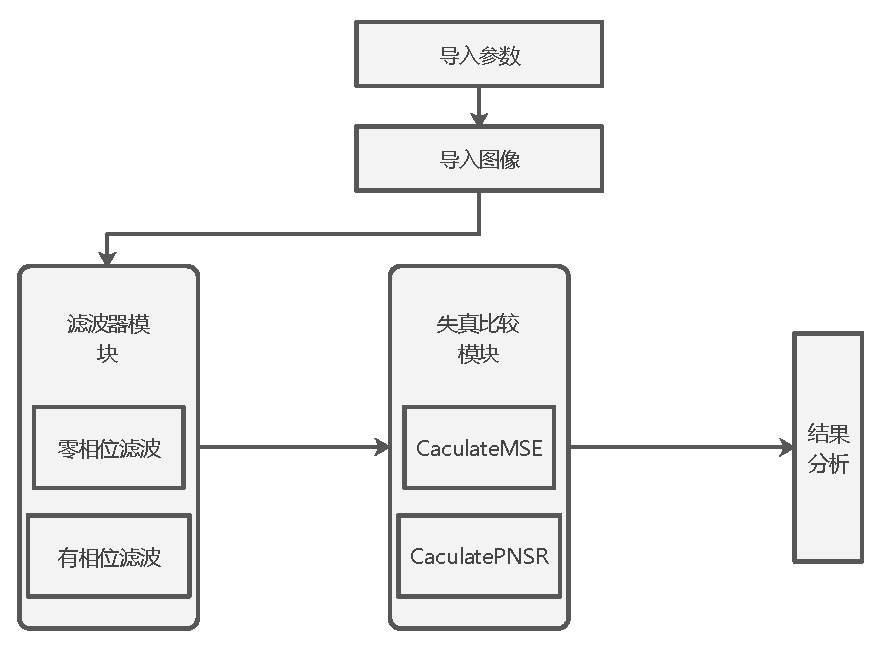
\includegraphics[width=10cm]{flowchart.eps}
    \caption{程序主要流程及模块图}
    \label{fig:flowchart}
\end{figure}

图\ref{fig:flowchart}展现了编程的主要模块与流程,我们将参数导入后生成题干中所描述的滤波器,之后又引入计算失真程度的失真比较模块比较不同滤波器在处理图像后的效果。同时我们也进一步分析了引起这种差异造成的原因。
\subsection{结果分析}

\subsubsection{第二问结果分析}
第二问要求我们考察三个滤波器的幅度与相位响应,通过Matlab中的freqz()函数即可得到频域谱。
\begin{figure}[h]
    \centering
    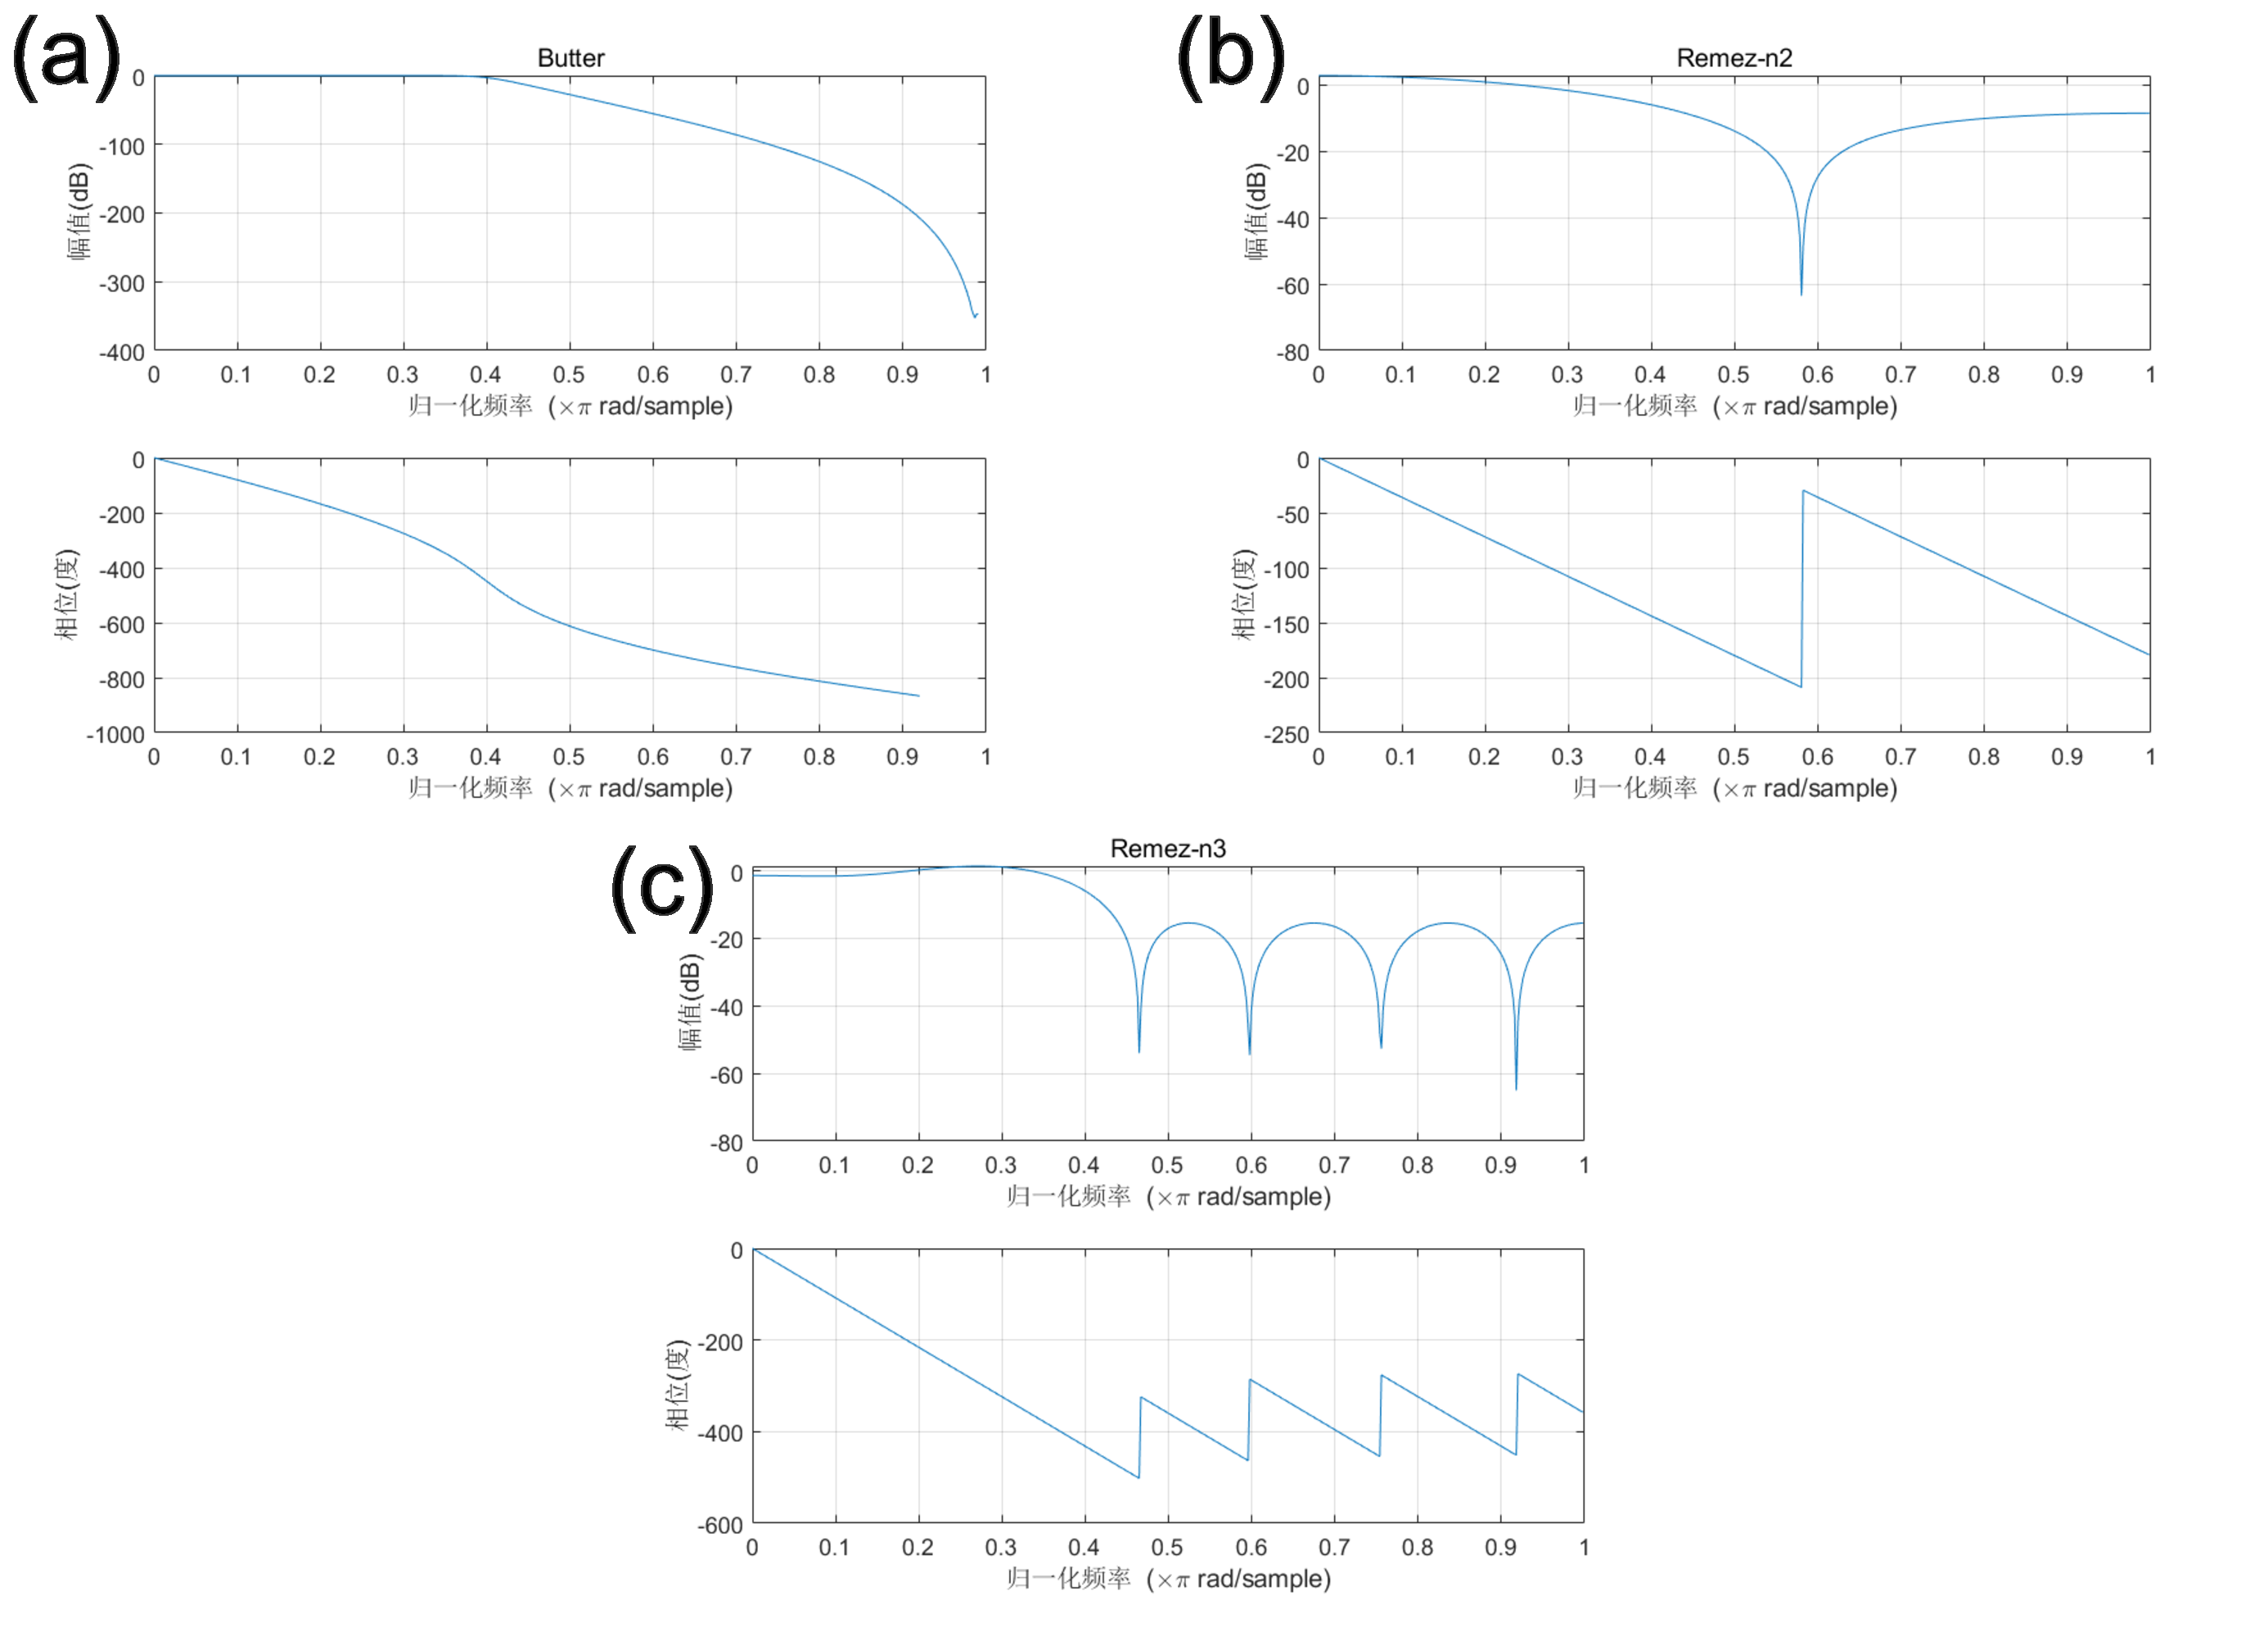
\includegraphics[width=10cm]{lvboxiangwei.eps}
    \caption{三种滤波器的幅度与相位谱}
    \label{fig:xiangwei}
\end{figure}

图\ref{fig:xiangwei}(a)展示了Butter滤波器的幅度谱与相位谱(以伯德图形式),其幅度谱为一条逐渐下降的曲线,表明该滤波器可以过滤较高的频率。而相位谱为一条平滑的曲线逐渐下降,表现出时域的平移。图\ref{fig:xiangwei}(b)展示了n2阶的Remez滤波器的相位谱与幅度谱,幅度谱展示了该滤波器在归一化后的截止频率为0.6左右的过滤效果较好,而相位谱在一定范围内为一条直线,说明通过该滤波器后相位并没有失真。图\ref{fig:xiangwei}(c)展示了n3阶Remez滤波器的相位谱与幅度谱,其相位与幅度谱均呈现锯齿形,从幅度谱上看,这表明该滤波器在不同范围的频率有着类似于周期性的滤波效果。从相位谱上看,对于超出对应归一化频率的部分,可能会造成信号的部分相位失真。由于n3>n2,即(c)显示出的滤波器阶数更高,所引起的相位失真可能更大。
\subsubsection{第三问结果分析}
通过导入第一问的参数,得到三种滤波器,分别画出三种滤波器随时间变化的响应如图\ref{fig:xiangying}所示。
\begin{figure}[h]
    \centering

    \includegraphics[width=8cm]{xiangying.jpg}
    \caption{三种滤波器的阶跃响应}
    \label{fig:xiangying}
\end{figure}


图\ref{fig:xiangying}显示了三种滤波器的单位阶跃响应,可以看出Butter(巴特沃斯)类型的滤波器具有明显的波动现象,而以n2为滤波器阶数的Remez(切比雪夫)滤波器则展现了良好的平滑性,难以直观的从图像中看到明显的波动;以n3为阶数的Remez滤波器则显示出幅度较小的振荡。


响应的超调为最大值与稳态值的差,通过令时间$t$趋向于无穷即可得到稳态值,而超调值=最大值-稳态值,计算得到三种滤波器超调后的结果如下表所示:
\begin{center}
\begin{table}[h]
\caption{三种滤波器的超调值}
\centering
\begin{tabular}{cc}
\toprule[1.5pt]
\makebox[0.2\textwidth][c]{滤波器名称} & \makebox[0.2\textwidth][c]{超调值}\\
\midrule[1pt]
Butter & 0.2165 \\
Remez-n2 & 0\\ 
Remez-n3 & 0.1275\\
\bottomrule[1.5pt]
\end{tabular}
\end{table}
\end{center}

从表中可以看出,巴特沃斯滤波器展示出了最大的超调值,为0.2165,其次为n3阶切比雪夫滤波器,最后为n2阶切比雪夫滤波器,超调值为0。这反映出巴特沃斯滤波器具有更大的不稳定因素,在实际应用中这种情况下的滤波器很难实现对系统的精确控制,而n2阶切比雪夫滤波器效果较好,可以实现稳定控制。
\subsubsection{第四、六问结果分析}
第四、六问类似,需要我们分别对x与xn图像进行同样的操作,图\ref{fig:boxlv}展示了两个图像分别经巴特沃斯滤波器、n2阶切比雪夫滤波器、n3阶切比雪夫滤波器经行、列滤波之后的结果。

\begin{figure}[h]
    \centering
    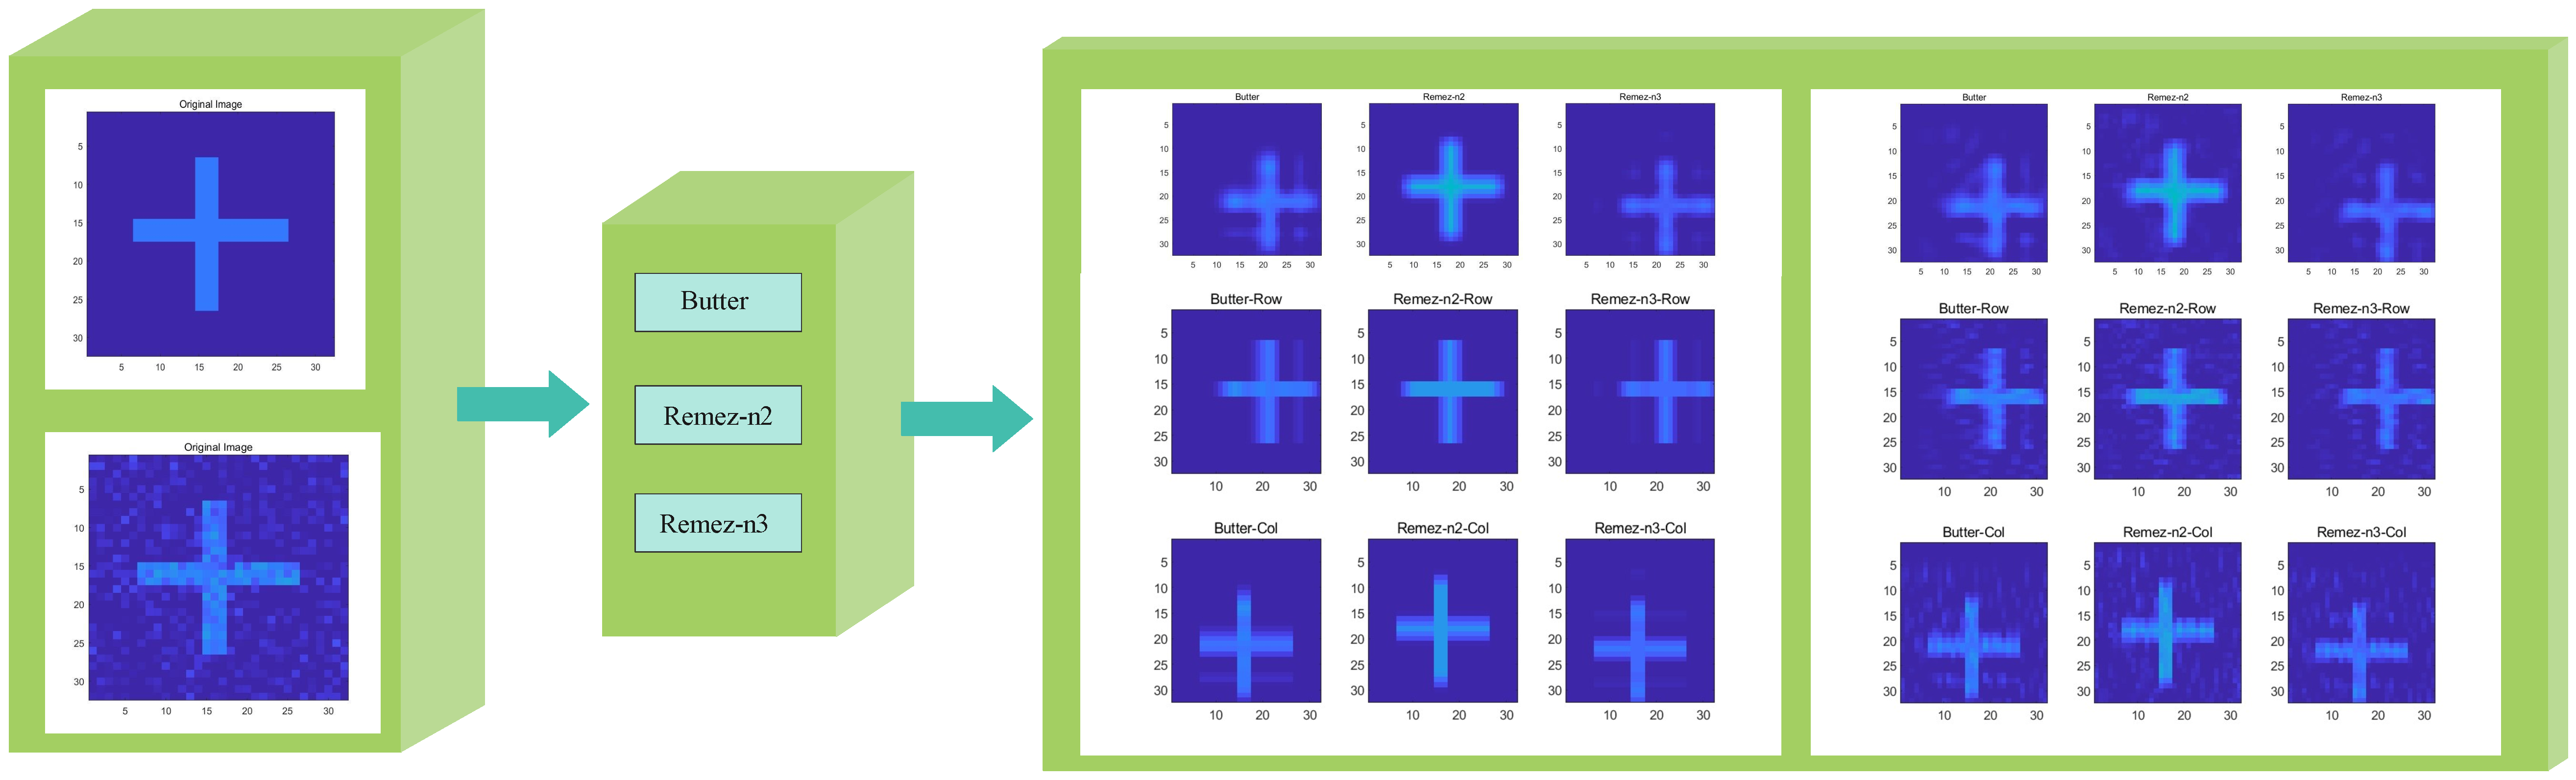
\includegraphics[width=14cm]{lvlv.eps}
    \caption{x与xn经行、列分别滤波后的图像与变化后的相位图}
    \label{fig:boxlv}
\end{figure}


图\ref{fig:boxlv}的左半部分展示了原始的x与xn图像,可以看出为一“十字形”,位于整个图像的中央。经过滤波器滤波之后的结果在右半部分展示出。图\ref{fig:boxlv}右半部分为x与xn滤波之后的图像。每个图的第一行与第二行分别展示了巴特沃斯滤波器、n2阶切比雪夫滤波器、n3阶切比雪夫滤波器对行、列同时或者分别进行滤波后的结果。巴特沃斯滤波器对行进行滤波后,会使原本图像的十字形向右进行偏移;对列滤波后则会使其向下偏移。n2阶切比雪夫滤波器则并未并未表现出明显的偏移现象。n3阶切比雪夫滤波器则展现出来了与巴特沃斯滤波器类似的效应,使得中心的十字分别向右或者向下偏移。而对x或者xn同时进行滤波后,可以看出图像的偏移为行滤波与列滤波叠加之后的效果。

为了定量比较图像的振荡,我们通过滤波后图像与原始图像的MSE与PNSR进行比较,刻画不同滤波器滤波偶的图像与原始图之间的差异性。
\begin{center}
\begin{table}[h]
\caption{图像x的振荡状况}
\label{tab:xshizhen}
\centering
\begin{tabular}{cccc}
\toprule[1.5pt]
\makebox[0.2\textwidth][c]{} &\makebox[0.2\textwidth][c]{Butter}& \makebox[0.2\textwidth][c]{Remez-n2}&\makebox[0.2\textwidth][c]{Remez-n3}\\
\midrule[1pt]
行、列滤波后的MSE& 681.0799&762.3861 &570.7006\\
行滤波后的MSE & 471.7019 & 319.8291&473.0550\\
列滤波后的MSE & 471.7019 & 319.8291 &473.0550\\ 
行、列滤波后的PNSR&7.7916 & 7.3018 & 8.5595 \\
行滤波后的PNSR &9.3869 &  11.0744&9.3745  \\
列滤波后的PNSR &9.3869 &11.0744& 9.3745  \\
 % 715.0163  847.0419  589.5562
\bottomrule[1.5pt]
\end{tabular}
\end{table}
\end{center}


表\ref{tab:xshizhen}展示了x图像的振荡情况,MSE越大,则反映图像图像有更为多的振荡,PNSR越小,则说明振荡越高。我们可以看出,通过巴特沃斯滤波器后展示了更为大的MSE,反映了与原始图像具有更大的差异。而n3阶切比雪夫滤波器则展示了更小的PNSR值,说明从这个角度来看,它与原始图像的差异更大,有更多的振荡。且同时对图像进行行列滤波后的结果也比分别对行、列进行滤波引入了更多的振荡。这个结果与图\ref{fig:boxlv}是吻合的。

\begin{center}
\begin{table}[h]
\caption{图像xn的振荡状况}
\label{tab:xnshizhen}
\centering
\begin{tabular}{cccc}
\toprule[1.5pt]
\makebox[0.2\textwidth][c]{} &\makebox[0.2\textwidth][c]{Butter}& \makebox[0.2\textwidth][c]{Remez-n2}&\makebox[0.2\textwidth][c]{Remez-n3}\\
\midrule[1pt]
行、列滤波后的MSE&715.0163 & 847.0419 & 589.5562\\
行滤波后的MSE & 513.5968 & 395.0001&516.3716\\
列滤波后的MSE & 557.6231 & 432.3848 &545.9817\\ 
行、列滤波后的PNSR& 7.5804 &6.8446 &8.4183\\
行滤波后的PNSR &9.0174 &  10.1576 &8.9940  \\
列滤波后的PNSR &8.6602  &9.7649&   8.7518  \\
 % 715.0163  847.0419  589.5562
 
% 三个图像与原本没有噪声图像的PNSR
    % 7.5804    6.8446    8.4183
\bottomrule[1.5pt]
\end{tabular}
\end{table}
\end{center}
% 9.0174    8.6602   10.1576    9.7649    8.9940    8.7518


表\ref{tab:xnshizhen}展示了xn图像的振荡情况,巴特沃斯对xn进行列滤波展现了最大的MSE与最小的PNSR值,则表明对于xn来说,巴特沃斯列滤波会引起更多的振荡。而n2阶切比雪夫滤波器在三个滤波器中则具备更小的MSE与更大的PNSR,表明通过此滤波器的图像与原始图像x更为接近,在三个滤波器中效果最好。

图像行列发生的变化是由于滤波器原本的相位影响,这使得图像行、列滤波后相位变化,,这导致图像在横向或者纵向上进行了平移。
\subsubsection{第五问结果分析}
图像的对称性发生破坏是相位失真的原因,跟据四、六问的分析可知,n3阶切比雪夫滤波器引入了更多的相位失真,对图像的对称性造成了很大的破坏。
\begin{figure}[h]
    \centering
    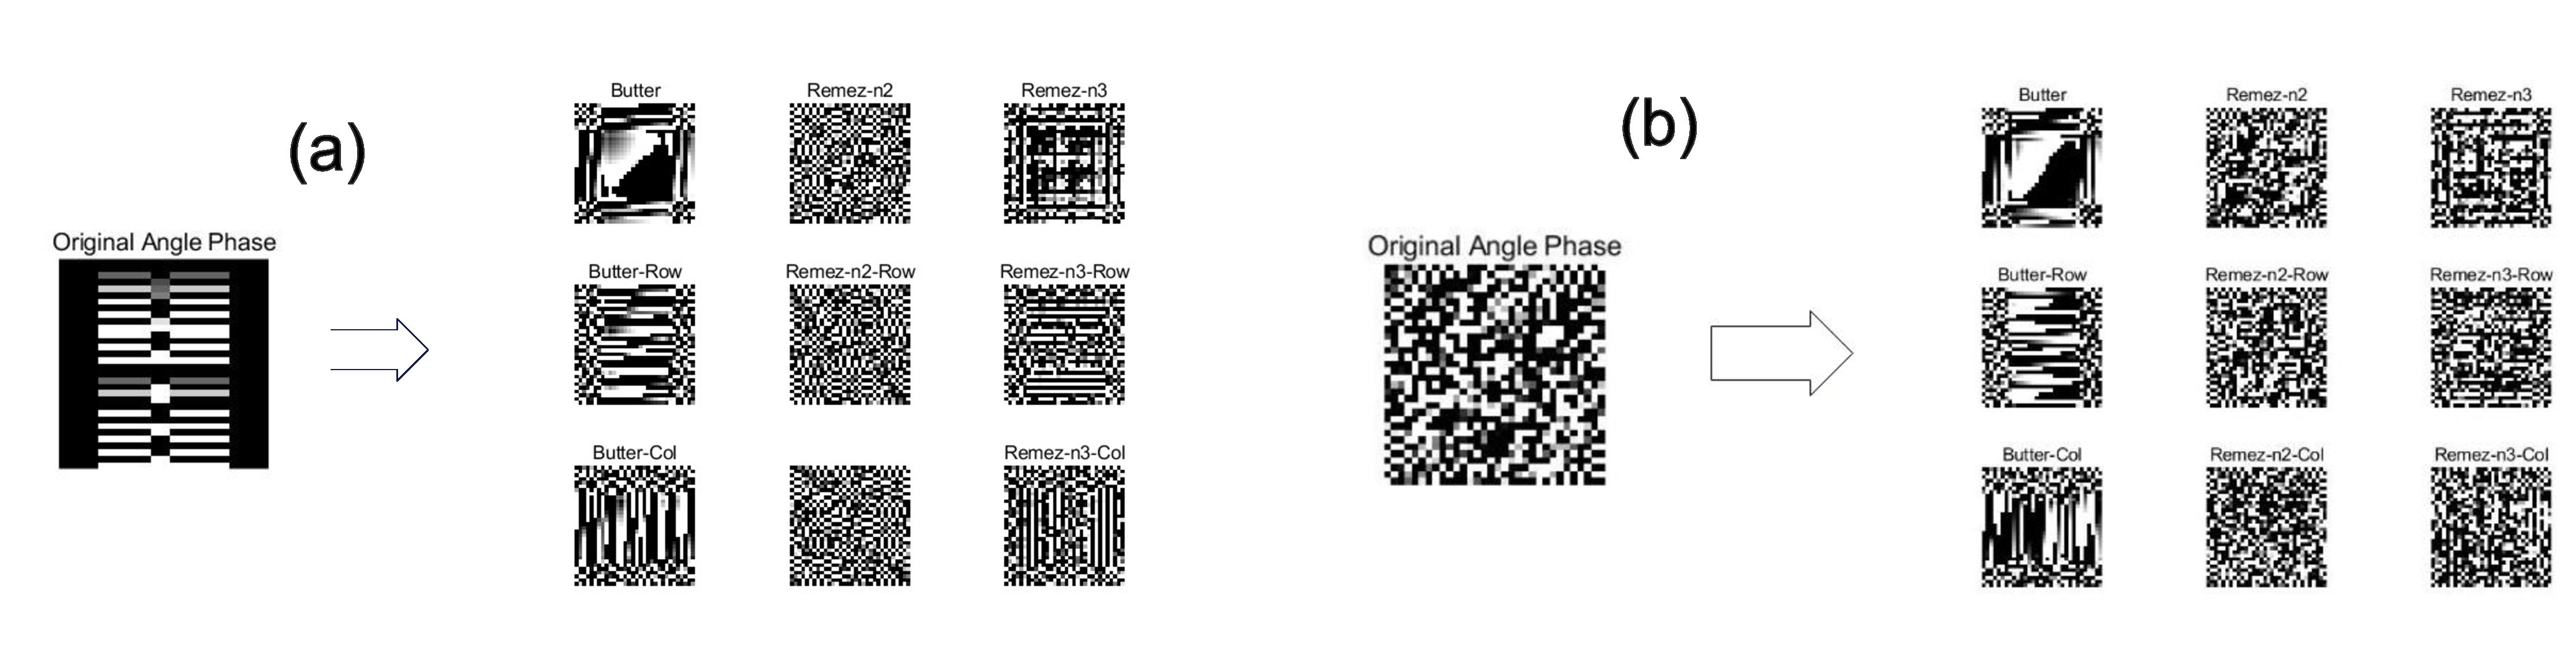
\includegraphics[width=14cm]{xiangwei.eps}
    \caption{x与xn经过九种滤波器后的相位谱变化}
    \label{fig:xi}
\end{figure}

图\ref{fig:xi}展示了图x与xn经过九种滤波器后的图像相位谱的变化,图像的相位谱反映了原本图像的轮廓与位置信息。虽然从现在的图中来看,图像的相位谱很像噪声特别是Remez-n2滤波器,但是却蕴含了复杂的轮廓与位置信息。图\ref{fig:xi}(a)展示了图像x的相位谱变化,图\ref{fig:xi}展示了图像xn的相位谱变化。在一维信号中,相位的平移(phase shift)在时域中引起原本信号中各分量之间对应的相位关系发生改变。而在二维图像中,我们很容易的可以递推得到如下类似公式:
\begin{equation}
\label{equ:xiange}
\varangle Y(e^{j\omega_1}, e^{j\omega_2})=\varangle X(e^{j\omega_1}, e^{j\omega_2}) + \varangle H(e^{j\omega_1}, e^{j\omega_2})
\end{equation}
式\ref{equ:xiange}展示中$\varangle Y(e^{j\omega_1}, e^{j\omega_2})$表示输出图像的相位角,$\varangle X(e^{j\omega_1}, e^{j\omega_2})$、$\varangle H(e^{j\omega_1}, e^{j\omega_2})$分别表示输入图像与系统的频率响应的相位角。我们通过一维滤波器处理二维图像,及首先对图像的每一行进行滤波,这导致图像行方向上相位谱的改变,如\ref{fig:xi}(a)(b)的第二行所示,同样的,如果先对列进行滤波则会导致图像每一列方向上的相位改变,如图\ref{fig:xi}(a)(b)的第三行所示。

为了进一步探究引起相位改变的原因,我们分别对三种滤波器在行、列与行列同时滤波后的单位冲激响应进行分析。对于一维信号而言,其单位冲激响应为冲激信号卷积系统函数,但是对于本研究而言,我们分别对行、列进行滤波,这种情况下的单位冲激信号等效于从行、列上来看都是单位冲击信号,即矩阵$\delta(m,n)$满足:
\begin{equation}
    \delta(m,n)=\left\{
\begin{aligned}
1& ,m=1\ or \ n=1\\
0& ,else
\end{aligned}
\right.
\end{equation}
其中$m$表示行,$n$表示列。

进一步地,我们将此二维情形下的单位冲击矩阵导入三种滤波器,并分别进行行、列与行列同时滤波,得到九种情况下的单位冲激响应与对应匹配的相位值,如图\ref{fig:5pp}所示。
\begin{figure}[h]
    \centering
    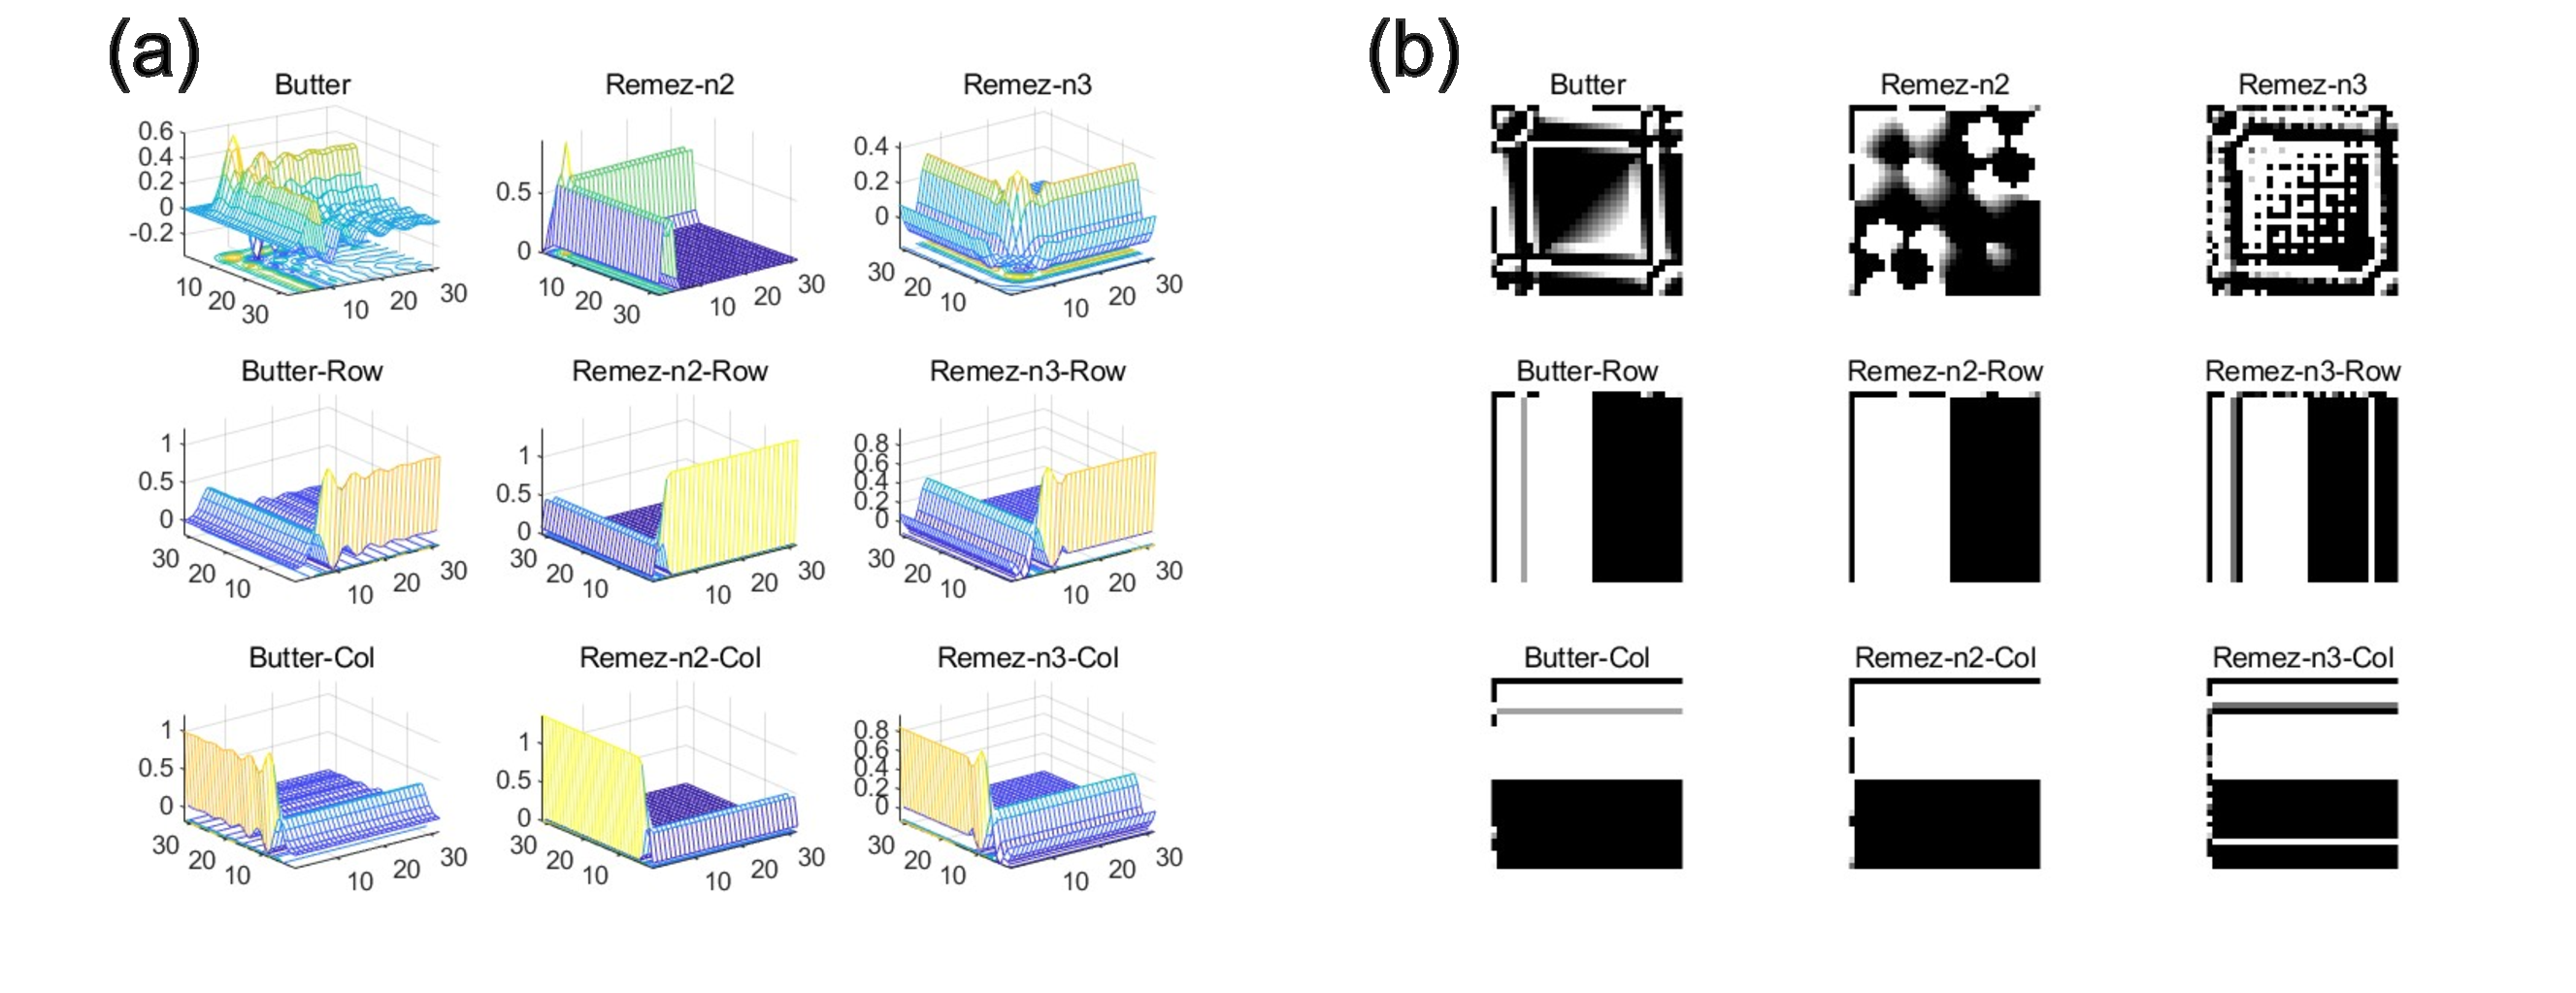
\includegraphics[width=14cm]{5pp.eps}
    \caption{九种情况下的单位冲击响应与相位图}
    \label{fig:5pp}
\end{figure}

图\ref{fig:5pp}(a)表示九种情况下的单位冲击响应,(b)则为对应的相位谱。图\ref{fig:5pp}(b)的相位谱对频率较高的部分进行了时移,反映到图像中即是对x或者xn的中心“十字”进行了响应的平移。以Butter滤波器为例,在频率更高的部分出现了更大的相位角(归一化后白色代表1,黑色代表0),这会让原本的图像有向右或者向下平移的趋势,这与在一维滤波的情况下是一致的。对于n2阶切比雪夫滤波器而言,由于其相位角的变化相对更小(图\ref{fig:xiangwei}所示),滤波后的图像并未具备明显的偏移现象。
\subsubsection{问题拓展}
至此,我们基本完成了大作业中所体现出的任务,但到这里我们很自然地联想到另一个问题。n2阶切比雪夫滤波器所产生的滤波效果较好是因为其时移现象较不明显,但如果我们对三种滤波器的时移情况进行削减,即三种滤波器的时移都不明显的话,那么效果最好的还依然是n2阶切比雪夫滤波器吗?

为了进一步研究在无时移情况下三种滤波器的效果如何,我们考虑如下方案:将原本的信号穿过滤波器后反向,再次穿过滤波器,两次滤波所引起的相位变化相互抵消,即可实现无时移传输滤波。但随之也会造成原本的信号激化过大,滤波器的阶数比原本的要高,即实现加倍。这里我们忽略滤波器阶数加倍而引起的影响,这并不会直接影响我们之后的分析结果。

将xn通过三种滤波器实现无时移的滤波,因为图像大小的限制,我们选取n3=10才有足够的样本进行反向滤波操作,滤波后的结果如图\ref{fig:wushiyi}所示。
\begin{figure}[h]
    \centering
    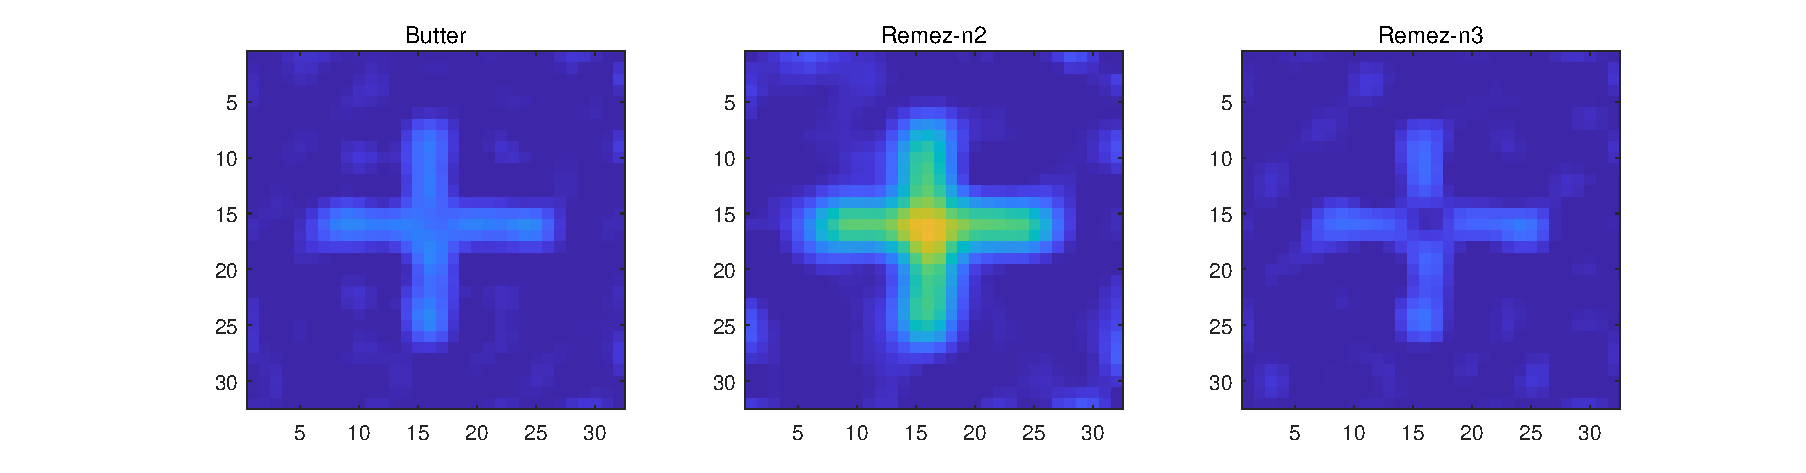
\includegraphics[width=14cm]{wuxiang.eps}
    \caption{无时移情况下的滤波结果}
    \label{fig:wushiyi}
\end{figure}

图\ref{fig:wushiyi}展示了无时移情况下的滤波结果,可以看出图像中心的“十字”没有偏移,这表明这种方式可以很好的抵消滤波器对相位变化造成的影响。此外,图\ref{fig:wushiyi}显示了Remez-n2滤波器的中心“十字”的颜色更深,其值更大,产生了较为明显的锐化现象,而其他两种滤波器的锐化现象则并不那么明显。
\begin{center}
\begin{table}[h]
\caption{无时移滤波后的振荡程度比较}
\label{tab:wushiyi}
\centering
\begin{tabular}{cccc}
\toprule[1.5pt]
\makebox[0.2\textwidth][c]{} &\makebox[0.2\textwidth][c]{Butter}& \makebox[0.2\textwidth][c]{Remez-n2}&\makebox[0.2\textwidth][c]{Remez-n3}\\
\midrule[1pt]
行、列滤波后的MSE&87.2 & 1561.4 & 179.8\\
行、列滤波后的PNSR& 16.7197 &4.1885&13.5758\\
\bottomrule[1.5pt]
\end{tabular}
\end{table}
\end{center}

上表\ref{tab:wushiyi}表明了滤波后的图像与原始图像的差异,与原本不同的地方在于,原本效果最好的Remez-n2(n2阶切比雪夫滤波器)在这里的效果最差,甚至远远差于其他的两种滤波器,而无时移的Butter滤波器则显示出了最好的效果,是在目前为止的讨论中效果最好的滤波器。

这充分的显示出滤波器对图像相位的影响会很大程度上影响我们滤波的效果。由于滤波器的相位,对原本图像进行过大的移动会很大程度上破坏图像原本具有的某些特性,这会导致某些坏的结果。
\newpage
\section{组内互评}
\begin{center}
\begin{table}[h]
\caption{评价表}
\centering
\begin{tabular}{cc}
\toprule[1.5pt]
\makebox[0.2\textwidth][c]{姓名} & \makebox[0.2\textwidth][c]{评分}\\
\midrule[1pt]
袁博文 &A\\ 
孙鹏卓 &B\\ 
ChatGPT &C\\
时圣铭 &D\\
王愉哲&D\\
\bottomrule[1.5pt]
\end{tabular}
\end{table}
\end{center}
任务完成情况:
\begin{itemize}
    \item 袁博文:Latex框架搭建,完成数学模型、程序编写,程序设计部分,修改并撰写第1,4部分论文。
    \item 孙鹏卓:完成数学模型部分,修改并完成第1,3部分论文撰写与论文查询方面工作。
    \item ChatGPT: 完成论文查询工作,并给出第1,6部分草稿。
    \item 时圣铭:使用ChatGPT提供第1部分初稿,完成第2部分撰写。
    \item 王愉哲:使用ChatGPT提供第6部分初稿。
\end{itemize}

\section{总结与体会}
最近,我们团队完成了基于一维滤波器的图像处理的大作业。每个人都在这次大作业中付出了很多也收获了很多。

作业让我们收获了很多技能方面的训练,比如我们尝试使用Overleaf协作进行文档编辑,这大大提高了我们的协作效率,比单独一个人用Word编写方便很多并且美观很多。此外,我们也对Matlab的图像处理模块与信号处理有了新的认识。

通过本次的工程作业,我们了解到,一维滤波器在图像、声音、生物等方面的作用。此外,原本在《信号与系统》中学习到关于滤波方面的知识也得到了体现,我们明白了原来一维滤波器的相位变化会对滤波后的效果产生十分大的影响,原来图像滤波器的相位谱图像十分重要,尽管难以直观的看出一些比较明显的信息,但却蕴含了相位,轮廓方面的信息。相位谱往往比幅度谱更为重要。

最后,我们的论文、代码均放在GitHub中开源,希望老师在明年的教学中可以让同学们尝试使用Latex编写论文,这绝对对他们十分有益。相关的Latex模板可以参考我们的main.tex文件。


\newpage
\bibliography{ref}
\addcontentsline{toc}{section}{参考文献}
\end{document}
